\documentclass[conference]{IEEEtran}

% para correr / compilar 
% pdflatex main.tex
% bibtex main
% pdflatex main.tex
% pdflatex main.tex
% 

\usepackage[spanish]{babel}
\usepackage{amsmath,amssymb,amsfonts,amsthm}
\usepackage[utf8]{inputenc} % Caracteres en Español (Acentos, ñs)
\usepackage{csquotes}
\usepackage{graphicx}
\usepackage{url} % ACENTOS
\usepackage{hyperref} % Referencias
\usepackage{subfig}
\usepackage{lipsum}
\usepackage{balance} 
\usepackage{etoolbox}
\usepackage{datetime}
\usepackage{float}
\makeatletter
\patchcmd{\frontmatter@RRAP@format}{(}{}{}{}
\patchcmd{\frontmatter@RRAP@format}{)}{}{}{}
\makeatother	

\usepackage[backend=bibtex,sorting=none]{biblatex}
\setcounter{biburllcpenalty}{7000}
\setcounter{biburlucpenalty}{8000}
\addbibresource{references.bib}

% fecha
\usepackage{datetime}
\newdateformat{specialdate}{
    \twodigit{\THEDAY}-\twodigit{\THEMONTH}-\THEYEAR
}
\date{\specialdate\today}

% la sentencia \burl en las citas... 
\usepackage[hyphenbreaks]{breakurl}
\renewcommand\spanishtablename{Tabla}
\renewcommand\spanishfigurename{Figura}


\begin{document}
% Definitions
\newcommand{\breite}{0.9} %  for twocolumn
\newcommand{\RelacionFiguradoscolumnas}{0.9}
\newcommand{\RelacionFiguradoscolumnasPuntoCinco}{0.45}

%Title of paper
\title{Reporte de Laboratorio X \\ Calculadora de Horas}

% Trabajo Individual
\author{
    \IEEEauthorblockN{
        Ricardo Emmanuel Uriegas Ibarra\IEEEauthorrefmark{1}
        }
    % En caso de trabajos en equipo, poner a todos los autores 
    % en estricto ORDEN ALFABETICO
    %\author{\IEEEauthorblockN{Michael Shell\IEEEauthorrefmark{1},
    %Homer Simpson\IEEEauthorrefmark{1}}
    \IEEEauthorblockA{
        \IEEEauthorrefmark{1}Ingeniería en Tecnologías de la Información\\
        Universidad Politécnica de Victoria
    }
}

\maketitle

%%%%%%%%%%%%%%%%%%%%%%%%%%%%%%%%%%%%%%%%%%%%%%%%%%%%%%%%%%%%%%%%%%%%%%%
\begin{abstract} 
    Dada la necesidad de calcular intervalos de tiempo con una aplicación que use una interfaz Qt6. En este trabajo se presenta el desarrollo de una aplicación denominada "Calculadora de Horas", implementada en el lenguaje de programación Python utilizando la librería PyQt6. La aplicación facilita el cálculo del tiempo transcurrido entre dos fechas y/o horas. Se realizaron pruebas para validar la precisión de los cálculos, obteniendo resultados consistentes con otras herramientas similares disponibles en línea\cite{calculator}.
\end{abstract}

%%%%%%%%%%%%%%%%%%%%%%%%%%%%%%%%%%%%%%%%%%%%%%%%%%%%%%%%%%%%%%%%%%%%%%%
\section{Introducción}
    En la actualidad, el cálculo de intervalos de tiempo es una tarea común en diversas áreas de la vida; desde la administración de proyectos, la programación de tareas, hasta la planificación de eventos. En este sentido, el desarrollo de una aplicación que permita calcular intervalos de tiempo de manera fácil se vuelve en algo de utilidad. En este trabajo se presenta el desarrollo de una aplicación en el lenguaje de programación Python y haciendo uso de la librería PyQt6. La aplicación permite el cálculo del tiempo transcurrido entre dos fechas y/o horas.

%%%%%%%%%%%%%%%%%%%%%%%%%%%%%%%%%%%%%%%%%%%%%%%%%%%%%%%%%%%%%%%%%%%%%%%
\section{Desarrollo Experimental}
    En este trabajo se desarrolló una aplicación calculadora de horas, con 2 diferentes formas de calcular el tiempo: usando una fecha con hora o solamente horas. Por defecto, la aplicación toma la fecha y hora actual del sistema operativo y las coloca en las entradas; esto para evitar colocar el botón \textit{Now} que tiene la aplicación de la página de calculator.net\cite{calculator} de la cual se inspiro nuestro proyecto.

    Se usan 3 diferentes tipos de entradas de entrada para evitar errores de validación en los datos; para las horas se usa una entrada tipo \textit{QTimeEdit}, para las fechas y horas se usa una entrada tipo \textit{QDateTimeEdit} y para el mostrado de resultados se usa una entrada tipo \textit{QPlainTextEdit} con la propiedad \textit{readOnly} activada, para asi deshabilitar la edición del texto en ella.

    \subsection{Método de Cálculo}
        Calcular el tiempo entre dos horas o fechas implica tomar los valores de inicio (\( t_{\text{inicio}} \)) y fin (\( t_{\text{fin}} \)), calcular su diferencia y presentar el resultado en la interfaz gráfica\ref{fig:des}. A continuación, se describen los métodos utilizados para el calculo de la diferencia de horas y fechas.

    \subsubsection{Cálculo entre dos horas}
        La diferencia entre dos horas específicas se calcula con el siguiente procedimiento:

        \begin{enumerate}
            \item Validar que \( t_{\text{inicio}} < t_{\text{fin}} \). Si no se cumple, el rango es inválido.
            \item Obtener la diferencia en segundos (\( \Delta t \)).
            \item Convertir \( \Delta t \) a horas, minutos y minutos totales:
            \[
                \text{horas} = \frac{\Delta t}{3600} \quad 
            \]
            \[
                \text{minutos} = \frac{\Delta t \mod 3600}{60} \quad 
            \]
            \[
                \text{minutos totales} = \frac{\Delta t}{60}
            \]
        \end{enumerate}

        El resultado se muestra en horas, minutos y minutos totales.

    \subsubsection{Cálculo entre dos fechas y horas}
        Para calcular la diferencia entre dos fechas con hora, se realiza el siguiente procedimiento:
        
        \begin{enumerate}
            \item Validar que \( dt_{\text{inicio}} < dt_{\text{fin}} \). Si no se cumple, el rango es inválido.
            \item Obtener la diferencia en segundos (\( \Delta t_{\text{s}} \)).
            \item Convertir \( \Delta t_{\text{s}} \) a días, horas y minutos:
            \[
                \text{días} = \frac{\Delta t_{\text{s}}}{24 * 3600} \quad 
            \]
            \[
                \text{horas totales} = \text{días} \times 24 + \text{horas} \quad 
            \]
            \[
                \text{minutos totales} = \text{horas totales} \times 60 + \text{minutos}
            \]
        \end{enumerate}
        
        El resultado incluye la diferencia en días, horas, minutos y sus equivalencias en horas y minutos totales.
        

%%%%%%%%%%%%%%%%%%%%%%%%%%%%%%%%%%%%%%%%%%%%%%%%%%%%%%%%%%%%%%%%%%%%%%%
\section{Resultados}
    Bien, hablando de resultados. La aplicación se comporta de manera correcta, se realizaron pruebas con diferentes intervalos de tiempo y se compararon con la calculadora de la página de calculator.net\cite{calculator}. Los resultados obtenidos fueron consistentes con los de la calculadora en línea, lo que indica que la aplicación desarrollada es precisa y confiable como se muestra en la figura \ref{fig:res}.

    \begin{figure}[!ht]
        \centering
        \subfloat[Calculo de horas]{
            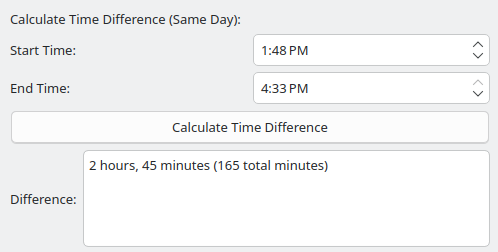
\includegraphics[width=0.45\textwidth]{images/horas.png}
            \label{fig:res1}
        }
        \hfill
        \subfloat[Calculo de fechas y horas]{
            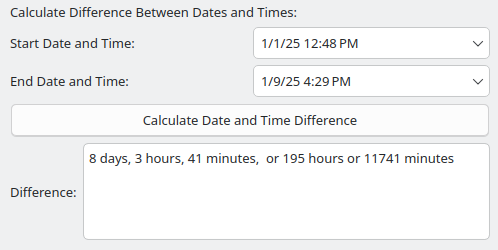
\includegraphics[width=0.45\textwidth]{images/fechas.png}
            \label{fig:res2}
        }
        \caption{Resultados de la aplicación.}
        \label{fig:res}
    \end{figure}

    En la figura \ref{fig:UI} se muestra el diseño resultante de la interfaz de usuario, donde se puede observar la entrada de fechas y horas, así como los botones para ejecutar el calculo del intervalo de tiempo, de igual manera se observa en \ref{fig:calendar} la selección de fechas (que es diferente a la selección de horas) cuyo propósito es facilitar al usuario una mas fácil entrada de datos. 

    En la figura \ref{fig:error2} se muestra el mensaje de error al ingresar una fecha de inicio mayor a la fecha de fin. De igual forma \ref{fig:error1} se muestra el mensaje de error al ingresar una hora de inicio mayor a la hora de fin.

    \begin{figure}[H]
        {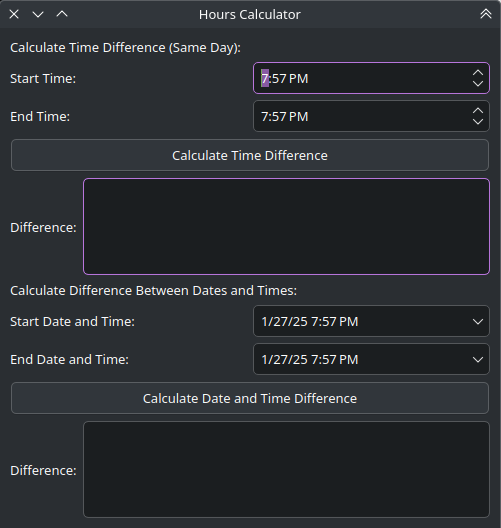
\includegraphics[width=\breite\columnwidth]{images/UI.png}}
        \caption{Interfaz general del usuario}
        \label{fig:UI}
    \end{figure}
    
    \begin{figure}[H]
        {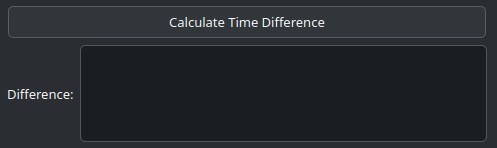
\includegraphics[width=\breite\columnwidth]{images/des.png}}
        \caption{Recuadro de texto deshabilitado donde se muestra la respuesta}
        \label{fig:des}
    \end{figure}
    
    % calendar.png
    \begin{figure}[H]
        {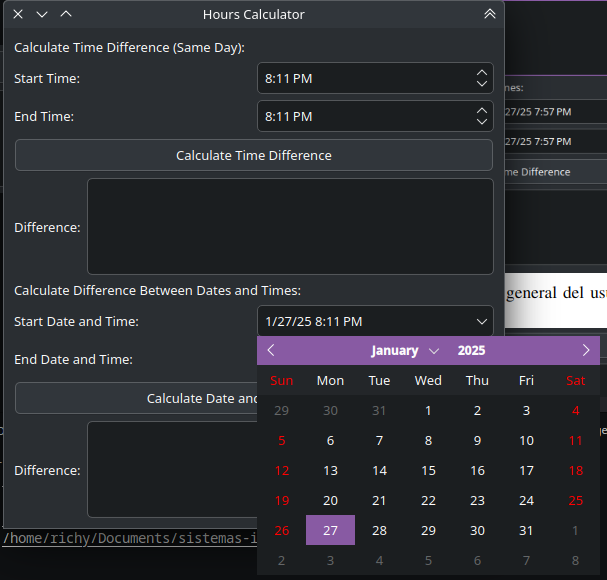
\includegraphics[width=\breite\columnwidth]{images/calendar.png}}
        \caption{Entrada de fechas y horas}
        \label{fig:calendar}
    \end{figure}
    
    % error1.png
    \begin{figure}[H]
        {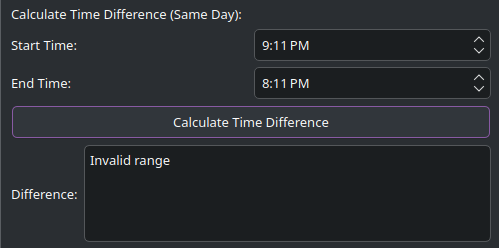
\includegraphics[width=\breite\columnwidth]{images/error1.png}}
        \caption{Mensaje de error al ingresar una fecha de inicio mayor a la fecha de fin}
        \label{fig:error1}
    \end{figure}
    
    % error2.png
    \begin{figure}[H]
        {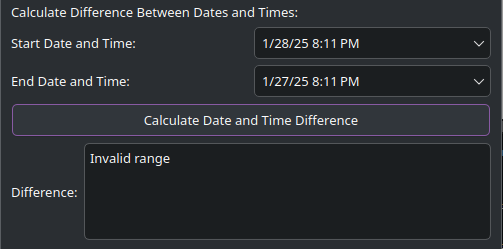
\includegraphics[width=\breite\columnwidth]{images/error2.png}}
        \caption{Mensaje de error al ingresar una hora de inicio mayor a la hora de fin}
        \label{fig:error2}
    \end{figure}

%%%%%%%%%%%%%%%%%%%%%%%%%%%%%%%%%%%%%%%%%%%%%%%%%%%%%%%%%%%%%%%%%%%%%%%
\section{Conclusión}
    En este trabajo se desarrolló una aplicación de calculadora de horas utilizando Python y PyQt6. Para lograrlo, se investigaron implementaciones de calculadoras en línea, tomando como referencia principal la calculadora de calculator.net. A partir de esta investigación, se diseñó una interfaz intuitiva que permite dos modos de cálculo principalmente; diferencia entre horas del mismo día y diferencia entre fechas con horas. La implementación se realizó utilizando widgets específicos de Qt como QTimeEdit y QDateTimeEdit para garantizar una entrada de datos válida. Los resultados obtenidos demuestran que la aplicación calcula correctamente los intervalos de tiempo, mostrando las diferencias en múltiples formatos (días, horas, minutos) y validando apropiadamente los rangos de tiempo ingresados. La aplicación cumple con todos los requisitos planteados y proporciona una solución sencilla para el cálculo de intervalos de tiempo.

%%%%%%%%%%%%%%%%%%%%%%%%%%%%%%%%%%%%%%%%%%%%%%%%%%%%%%%%%%%%%%%%%%%%%%%
\addcontentsline{toc}{section}{Referencias} 
\printbibliography
%\balance

\end{document}